\section{多目标问题}
\label{sec:moo-problem}

目标从一个数变成一组数之后，“更好”和“最优”还能怎样定义？本节先把问题写出来，再找出不需要任何偏好就能成立的比较，最后说明目标的单位会影响哪些判断。

\paragraph{问题的形式}
在同一个可行集上，同时要求$m$个目标都尽量小，这样的问题称为\term{多目标优化}（multi-objective optimization）：
\begin{equation}
 \min_{\bm{x}\in\bm{C}}\ \bm{f}(\bm{x})=\bigl(f_1(\bm{x}),\ldots,f_m(\bm{x})\bigr).
 \label{eq:moo-problem}
\end{equation}
本章的$m$始终表示目标个数。需要写约束函数时，第~\ref{sec:moo-feasible-direction}节会另外安排下标。这里的“$\min$”暂时只是一个愿望，它的含义正是本节要确定的。

问题涉及两个空间。变量$\bm{x}$所在的$\mathbb{R}^n$称为\term{决策空间}（decision space），目标向量所在的$\mathbb{R}^m$称为\term{目标空间}（objective space）。可行集在$\bm{f}$下的像
\begin{equation}
 \bm{Y}=\bm{f}(\bm{C})=\{\bm{f}(\bm{x}):\bm{x}\in\bm{C}\}
 \label{eq:moo-reachable}
\end{equation}
是所有能够实现的目标向量，称为\term{可达目标集}（attainable objective set）。决定方案好坏的比较发生在$\bm{Y}$里，而真正要交出去的方案在$\bm{C}$里。

\paragraph{两个贯穿全章的例子}
第一个例子是有限个候选。六个方案的成本$f_1$（万元）和误差$f_2$（百分点）如下，数据是教学用的假设：
\begin{equation}
 \begin{gathered}
  A=(1,8),\quad B=(2,5),\quad C=(4,4),\\
  D=(6,1),\quad E=(5,6),\quad F=(7,1).
 \end{gathered}
 \label{eq:moo-candidates}
\end{equation}
这里决策空间就是六个方案的名字，目标空间是平面，$\bm{Y}$由六个点组成。

第二个例子是连续的。取$\bm{C}=\mathbb{R}^2$，两个目标分别希望靠近两个不同的点：
\begin{equation}
 f_1(\bm{x})=\frac12\lVert\bm{x}-\bm{a}\rVert_2^2,\qquad
 f_2(\bm{x})=\frac12\lVert\bm{x}-\bm{b}\rVert_2^2,
 \label{eq:moo-iso}
\end{equation}
其中$\bm{a}=(1,0)$，$\bm{b}=(0,1)$。想象两个仓库分别在$\bm{a}$和$\bm{b}$，要选一个地点，离两个仓库都要近。

图~\ref{fig:moo-two-spaces}把这个映射画了出来。左边是决策平面，右边是目标平面，浅蓝色区域是$\bm{Y}$。点$\bm{p}=(1,1)$与$\bm{p}'=(0,0)$关于直线$x_1+x_2=1$对称，到两个仓库的距离分别相同，所以落到目标平面上的同一点$(1/2,1/2)$。一个目标向量可以对应多个方案，这正是不能只在目标空间里回答“选哪个方案”的原因。

\begin{BookInlineFigure}
  \centering
  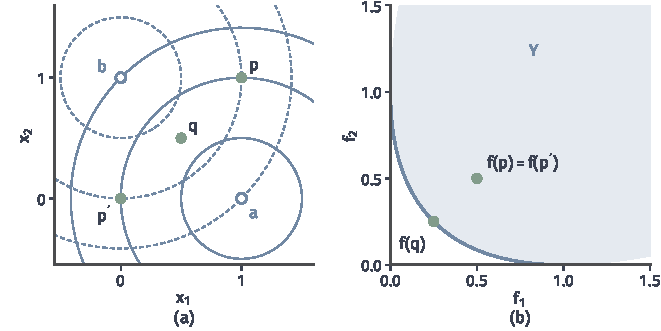
\includegraphics[width=112mm]{figures/05-optimization/07-multiple-criteria-and-nested-optimization/matplotlib/moo-two-spaces/figure.pdf}
  \caption{式~\eqref{eq:moo-iso}的决策空间与目标空间。(a)实线圆是$f_1$的等高线，虚线圆是$f_2$的等高线，绿点是三个方案。(b)浅蓝区域是可达目标集$\bm{Y}$，蓝线是它的左下边界。$\bm{p}$与$\bm{p}'$对称，映到同一个目标向量；$\bm{q}=(1/2,1/2)$的目标向量是$(1/4,1/4)$，两个分量都更小。}
  \label{fig:moo-two-spaces}
\end{BookInlineFigure}

\paragraph{为什么没有唯一的最小}
单目标问题中，任意两个实数都能比较大小，所以最小值的定义不会有歧义。向量没有这样的全序。$A=(1,8)$与$D=(6,1)$相比，成本是$A$小，误差是$D$小。两个分量的优劣方向相反，要断定谁更好，必须先说清一万元相当于多少个百分点的误差，而题目没有给出这个信息。

因此不能指望从式~\eqref{eq:moo-problem}直接得到一个点。接下来只保留不需要换算就能下的判断。

\subsection{支配关系}
\label{sec:moo-dominance}

不引入任何偏好，还能确定哪些比较？回到式~\eqref{eq:moo-candidates}，$B=(2,5)$与$E=(5,6)$相比，$B$更便宜，误差也更小。无论决策者多看重成本或多看重误差，只要两项都是越小越好，就没有理由选$E$。把这种“全面不差”写成定义。

\begin{definition}[支配]
\label{def:moo-dominance}
设$\bm{u},\bm{v}\in\bm{C}$。若
\begin{equation}
 f_i(\bm{u})\leq f_i(\bm{v})\quad\text{对所有}\ i=1,\ldots,m,
 \label{eq:moo-dom-weak}
\end{equation}
并且至少有一个$i$使$f_i(\bm{u})<f_i(\bm{v})$，就说$\bm{u}$\term{支配}（dominate）$\bm{v}$。
\end{definition}

式~\eqref{eq:moo-dom-weak}说的是“每一项都不差”，后半句说的是“至少有一项确实更好”。后半句不能省：没有它，两个目标向量相同的方案就会互相支配，而它们之间其实没有优劣。

\paragraph{用左下区域检查}
在目标平面上，支配关系可以一眼看出。以一点$\bm{y}$为角画出它的左下方区域和右上方区域，落在左下方的点支配$\bm{y}$，落在右上方的点被$\bm{y}$支配。图~\ref{fig:moo-dominance}(a)以$B$为例，平面被两条虚线分成四块。左上和右下两块中的点一个分量比$B$小，另一个分量比$B$大，这两块就是\textbf{不可比}的区域。

\begin{BookInlineFigure}
  \centering
  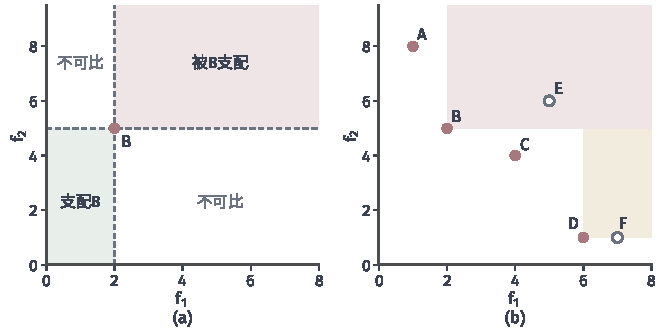
\includegraphics[width=112mm]{figures/05-optimization/07-multiple-criteria-and-nested-optimization/matplotlib/moo-dominance/figure.pdf}
  \caption{目标平面上的支配关系，数据为式~\eqref{eq:moo-candidates}。(a)以$B$为角分出的四块区域。(b)红点是不被任何候选支配的方案，空心点是被支配的方案。粉色是被$B$支配的区域，$E$在其中；浅黄是被$D$支配的区域，$F$在它的下边界上。}
  \label{fig:moo-dominance}
\end{BookInlineFigure}

下面逐对检查图~\ref{fig:moo-dominance}(b)中的六个点。$E=(5,6)$被$B$支配，也被$C=(4,4)$支配。$F=(7,1)$与$D=(6,1)$误差相同，$D$更便宜，所以$D$支配$F$。其余的$A,B,C,D$按成本从小到大排，误差依次是$8,5,4,1$，严格下降，任何两个都是一项更好、一项更差，互不支配。

支配是一种偏序：一个点不支配自己，支配关系可以传递，但并非任何两点都可比。可比的部分是确定的判断，不可比的部分要等偏好来决定。

\subsection{Pareto最优}
\label{sec:moo-pareto}

既然只有部分方案之间能比较，“最优”就只能退一步定义：没有被其他方案全面超过。这一小节给出这个定义及其两种变形，并把它们落到两个例子上。

\begin{definition}[Pareto最优]
\label{def:moo-pareto}
设$\bar{\bm{x}}\in\bm{C}$。
\begin{enumerate}
 \item 若不存在$\bm{x}\in\bm{C}$支配$\bar{\bm{x}}$，称$\bar{\bm{x}}$为\term{Pareto最优}（Pareto optimal）点。
 \item 若不存在$\bm{x}\in\bm{C}$使$f_i(\bm{x})<f_i(\bar{\bm{x}})$对所有$i$成立，称$\bar{\bm{x}}$为\term{弱Pareto最优}（weakly Pareto optimal）点。
 \item 若存在$r>0$，使上述条件在$\bm{C}$与$\bar{\bm{x}}$的$r$邻域的交集上成立，相应地称为\term{局部Pareto最优}（locally Pareto optimal）点或局部弱Pareto最优点。
\end{enumerate}
全体Pareto最优点组成的集合称为\term{Pareto解集}（Pareto set），记为$\bm{X}_{\mathrm{P}}$；它在$\bm{f}$下的像$\bm{Y}_{\mathrm{P}}=\bm{f}(\bm{X}_{\mathrm{P}})$称为\term{Pareto前沿}（Pareto front）。
\end{definition}

解集在决策空间，前沿在目标空间，二者不是同一个东西。多个方案可以对应前沿上的同一点，所以由前沿反推方案时还要保留决策变量。

未加“局部”二字的Pareto最优指全局版本，比较对象是全部可行点。全局Pareto最优点必定是局部Pareto最优点，因为比较的范围缩小了。Pareto最优点必定是弱Pareto最优点，因为所有分量都严格更小的点一定支配它。

\paragraph{有限例}
在式~\eqref{eq:moo-candidates}中，$A,B,C,D$都不被支配，都是Pareto最优点。$E$被$B$支配，且$B$的两个分量都严格小于$E$，所以$E$连弱Pareto最优点也不是。

$F=(7,1)$被$D$支配，因此不是Pareto最优点。可是要两个分量都严格小于$F$，误差必须小于$1$，而六个方案中没有这样的。所以$F$是弱Pareto最优点。弱Pareto最优这个说法宽松，正是因为它放过了“一项持平、另一项更差”的方案。

\paragraph{弱Pareto点在目标平面上的样子}
图~\ref{fig:moo-weak-pareto}中可达集合的边界有三段。红色曲线段上的点都是Pareto最优的。左侧的竖直边上，$\bm{y}$的左下方开象限（绿色）里没有可达点，所以$\bm{y}$是弱Pareto最优的；但沿着竖直边往下走到$\bm{y}'$，成本不变而误差变小，$\bm{y}'$支配$\bm{y}$。底部的水平边同理，$\bm{z}'$支配$\bm{z}$。

\begin{BookInlineFigure}
  \centering
  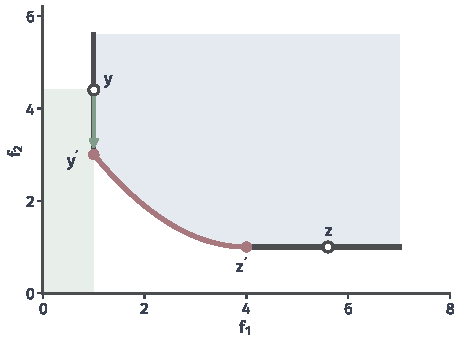
\includegraphics[width=78mm]{figures/05-optimization/07-multiple-criteria-and-nested-optimization/matplotlib/moo-weak-pareto/figure.pdf}
  \caption{弱Pareto最优点的位置。浅蓝区域是可达目标集，红色曲线是Pareto前沿，深灰粗线是只有弱Pareto性质的竖直边和水平边。绿色是$\bm{y}$的左下方开象限，其中没有可达点。绿色箭头指向支配$\bm{y}$的点$\bm{y}'$。}
  \label{fig:moo-weak-pareto}
\end{BookInlineFigure}

\paragraph{连续例：解集是一条线段}
现在求式~\eqref{eq:moo-iso}的Pareto解集。选坐标把几何关系拆开：把点写成沿$\bm{a}\to\bm{b}$的位置$s$与到连线的带符号距离$r$，
\[
 \bm{x}=\bm{a}+s(\bm{b}-\bm{a})+r\bm{e},\qquad \bm{e}=\tfrac{1}{\sqrt2}(1,1).
\]
由于$\bm{e}$是与$\bm{b}-\bm{a}$垂直的单位向量，且$\lVert\bm{b}-\bm{a}\rVert_2^2=2$，由勾股定理得到
\begin{equation}
 f_1=s^2+\tfrac12r^2,\qquad f_2=(1-s)^2+\tfrac12r^2.
 \label{eq:moo-iso-coords}
\end{equation}

式~\eqref{eq:moo-iso-coords}说明，三种情形下都能找到严格更好的点。若$r\neq0$，把$r$改为$0$，两个目标都严格减小。若$r=0$而$s<0$，把$s$改为$0$，$f_1$从$s^2$减为$0$，$f_2$从$(1-s)^2$减为$1$，两项都严格减小。$s>1$时对称。

所以Pareto最优点只可能在线段$s\in[0,1]$，$r=0$上。还要确认线段上的点确实不被支配。设$\bm{y}$支配线段上参数为$s$的点，按上面的做法把$\bm{y}$拉回线段得到参数$s'$，目标不增，于是$\bm{f}$在$s'$处的值逐项不大于在$s$处的值。

线段上$f_1=s^2$严格递增，$f_2=(1-s)^2$严格递减，两项同时不大于只能发生在$s'=s$。这样拉回前后目标向量相等，$\bm{y}$与原点目标相同，与“支配”矛盾。于是
\begin{equation}
 \bm{X}_{\mathrm{P}}=\{(1-s,s):0\leq s\leq1\},\qquad
 \bm{Y}_{\mathrm{P}}=\{(s^2,(1-s)^2):0\leq s\leq1\}.
 \label{eq:moo-iso-front}
\end{equation}

图~\ref{fig:moo-pareto-set-front}画出这一结果。线段外的点$\bm{p}=(1,1)$对应目标向量$(1/2,1/2)$，沿箭头移到$\bm{q}$后目标变成$(1/4,1/4)$，两项都减半。线段内部沿着线段移动，则是拿$f_1$换$f_2$，这种交换就是\term{取舍}（trade-off）的含义。

\begin{BookInlineFigure}
  \centering
  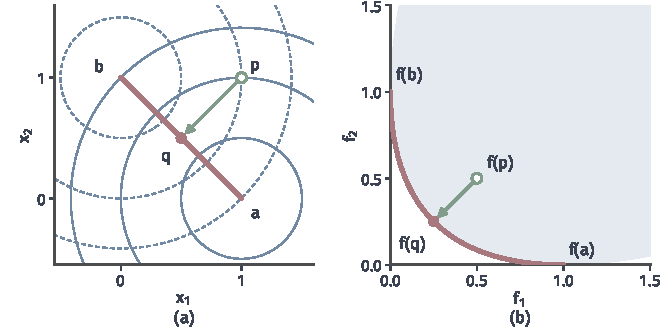
\includegraphics[width=112mm]{figures/05-optimization/07-multiple-criteria-and-nested-optimization/matplotlib/moo-pareto-set-front/figure.pdf}
  \caption{式~\eqref{eq:moo-iso}的Pareto解集与Pareto前沿。(a)决策平面上红色线段是解集，绿色箭头把线段外的点$\bm{p}$移到$\bm{q}$。(b)目标平面上浅蓝区域是可达目标集，红色曲线是前沿$(s^2,(1-s)^2)$；同一步移动使$\bm{f}(\bm{p})$沿箭头落到前沿上的$\bm{f}(\bm{q})$。}
  \label{fig:moo-pareto-set-front}
\end{BookInlineFigure}

\paragraph{局部版本与存在性}
局部Pareto最优只和附近的方案比。取一个变量$x\in[0,4]$，令
\begin{equation}
 f_1(x)=x,\qquad f_2(x)=(x-1)^2(x-3)^2+0.4x.
 \label{eq:moo-local}
\end{equation}
由于$f_1$随$x$增大，$x$越大的方案越贵，所以一个方案不被支配，要求所有更便宜的方案的误差都更大。

图~\ref{fig:moo-local-pareto}是这条曲线。$f_2$的第一个极小点约在$x\approx0.953$，记对应点为$\bm{P}$，$[0,0.953]$上的$f_2$严格下降，这一段是全局Pareto最优的（红色）。第二个极小点约在$x\approx2.946$，记对应点为$\bm{Q}$，通往$\bm{Q}$的紫色下降段上，近处更便宜的方案误差更大，近处更贵的方案误差更小，互不支配，所以这一段局部Pareto最优。

但$\bm{Q}$的两个分量约为$(2.946,1.189)$，$\bm{P}$的两个分量约为$(0.953,0.390)$，都更小，$\bm{P}$支配$\bm{Q}$。这和单目标问题中局部最小点与全局最小点的差别是一回事，只是这里比较的是向量。

\begin{BookInlineFigure}
  \centering
  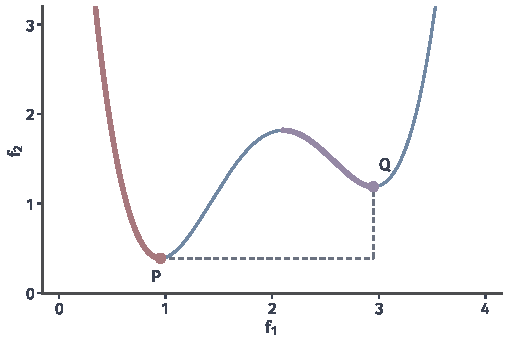
\includegraphics[width=86mm]{figures/05-optimization/07-multiple-criteria-and-nested-optimization/matplotlib/moo-local-pareto/figure.pdf}
  \caption{式~\eqref{eq:moo-local}在目标平面上的曲线。红色段全局Pareto最优，紫色段只局部Pareto最优，蓝色段的点在近处已被支配。虚线标出$\bm{P}$支配$\bm{Q}$的两个分量差。}
  \label{fig:moo-local-pareto}
\end{BookInlineFigure}

Pareto最优点也不是总存在的。取$\bm{C}=(0,1]$，$f_1(x)=f_2(x)=x$，任意$x$都被$x/2$支配，解集是空集。这和单目标问题中最小点不存在是同一种情形，第~\ref{sec:moo-scalarization}节会给出一个保证存在的条件。

\subsection{目标尺度}
\label{sec:moo-scale}

单位是人为选定的。把成本从万元换成千元，数字扩大十倍，这时哪些结论不变，哪些结论会变？

\paragraph{支配关系不受影响}
若把每个目标换成$\varphi_i(f_i)$，其中$\varphi_i$严格递增，那么$f_i(\bm{u})\leq f_i(\bm{v})$与$\varphi_i(f_i(\bm{u}))\leq\varphi_i(f_i(\bm{v}))$等价，严格不等号也一样。所以支配关系、Pareto解集、弱Pareto解集都不变。换单位是$\varphi_i(y)=cy$，$c>0$，自然在其中。

\paragraph{固定权重的加权目标会变}
把两个目标按固定权重相加，比如权重取$(0.6,0.4)$，得到一个分数，分数最低的方案胜出。以万元为单位，四个Pareto方案的分数是
\[
 A:\ 3.8,\qquad B:\ 3.2,\qquad C:\ 4,\qquad D:\ 4,
\]
所以选$B$。把成本改用千元表示，$f_1$乘以$10$，权重不变，分数变成
\[
 A:\ 9.2,\qquad B:\ 14,\qquad C:\ 25.6,\qquad D:\ 36.4,
\]
这回选$A$。方案本身什么也没变，变的只是记账单位，见图~\ref{fig:moo-scale-weight}。

\begin{BookInlineFigure}
  \centering
  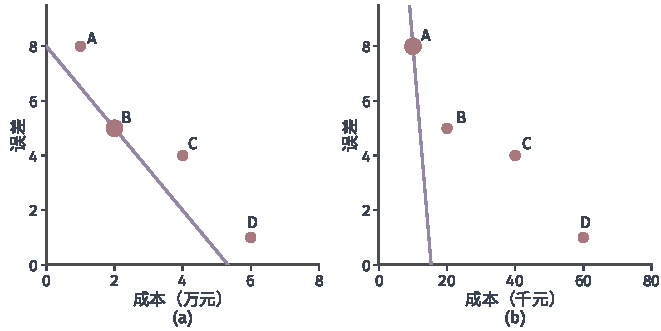
\includegraphics[width=112mm]{figures/05-optimization/07-multiple-criteria-and-nested-optimization/matplotlib/moo-scale-weight/figure.pdf}
  \caption{换单位改变加权和的选择，权重固定为$(0.6,0.4)$。紫线是经过分数最低方案的等分数线，大圆点是被选中的方案。(a)成本以万元计，选中$B$。(b)成本以千元计，选中$A$。四个点的相对位置在两图中按横轴比例对应，支配关系没有变化。}
  \label{fig:moo-scale-weight}
\end{BookInlineFigure}

\paragraph{基于距离的比较也会变}
另一种常见做法是计算到\term{理想点}（ideal point）的距离。理想点的每个分量是该目标单独能达到的最小值，这里是$(1,1)$。以万元为单位，四个方案到理想点的欧氏距离约为
\[
 A:\ 7,\qquad B:\ 4.12,\qquad C:\ 4.24,\qquad D:\ 5,
\]
$B$最近。改用千元后，理想点变为$(10,1)$，距离约为
\[
 A:\ 7,\qquad B:\ 10.77,\qquad C:\ 30.15,\qquad D:\ 50,
\]
$A$最近。距离把两个分量的差放在一起平方，单位大的分量就占了主导。

\paragraph{归一化及其参考范围}
为消除单位，常把每个目标按某个参考范围线性缩放到$[0,1]$。取目标$i$的下参考值$l_i$和上参考值$u_i$，$u_i>l_i$，令
\begin{equation}
 \tilde{f}_i=\frac{f_i-l_i}{u_i-l_i}.
 \label{eq:moo-normalize}
\end{equation}
下参考值常取理想点。上参考值常取Pareto方案中各目标的最大值，这样的点称为\term{最差点}（nadir point）。

以$A,B,C,D$的范围$l=(1,1)$，$u=(6,8)$归一化，四点变成
\[
 A:\ (0,1),\quad B:\ (0.2,0.571),\quad C:\ (0.6,0.429),\quad D:\ (1,0).
\]
到原点的距离依次约为$1$，$0.605$，$0.737$，$1$，选$B$。这一结果不再受万元或千元的影响，因为式~\eqref{eq:moo-normalize}的分子分母同时乘以同一个数。

但参考范围本身仍然影响结论。设候选集里多了一个$G=(1.5,36)$，它被$A$支配，本该无关紧要。若范围取全部候选的最大值，误差的上参考值变成$36$，四点的归一化误差都缩小，距离依次约为$0.2$，$0.230$，$0.606$，$1$，选中的方案从$B$变成$A$，见图~\ref{fig:moo-scale-range}。

\begin{BookInlineFigure}
  \centering
  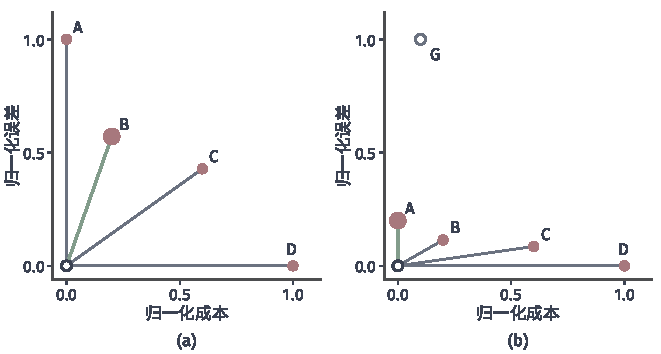
\includegraphics[width=112mm]{figures/05-optimization/07-multiple-criteria-and-nested-optimization/matplotlib/moo-scale-range/figure.pdf}
  \caption{参考范围对归一化比较的影响。线段是各方案到理想点（原点）的距离，绿色线段是最短的一条，大圆点是被选中的方案。(a)以$A,B,C,D$的范围归一化，选$B$。(b)候选中混入被支配的$G=(1.5,36)$，误差范围变大，选$A$。}
  \label{fig:moo-scale-range}
\end{BookInlineFigure}

这里的教训有两条。凡是用到权重或距离的比较，都要写明所用的单位或参考范围。归一化不是中性的操作，它把“一单位误差值多少钱”换成了“各目标范围的一格彼此相当”，这也是一种偏好，只是不那么显眼。参考范围最好由被信任的方案决定，并在结果中报告，不让被支配的候选参与定尺度。
